\documentclass{article}


\usepackage[T2A]{fontenc}
\usepackage[utf8]{inputenc}
\usepackage[russian]{babel}
\usepackage{float}

\usepackage[unicode, colorlinks, linkcolor=blue]{hyperref}

\usepackage{graphicx}
\graphicspath{{pictures/}}
\DeclareGraphicsExtensions{.pdf,.png,.jpg}

\usepackage{pgfplots}


\begin{document}
%----------------------------------Шапка---------------------------------------------
	\begin{center}
		
\includegraphics[scale=0.25]{AU}\\
		{\Large\bfseries Санкт-Петербургский национальный исследовательский Академический университет имени Ж.И.~Алфёрова Российской академии наук}
	\end{center}

	\begin{center}
		Свиридов Фёдор, Александр Слободнюк, Владимир Попов
	\end{center}
	\rule{12cm}{0.4mm}
	\begin{center}
		{\large\textbf{Рабочий протокол и отчёт по лабораторной работе № 4}}
	\end{center}
%--------------------------------------------------------------------------------------
\paragraph{Цель работы.}
С помощью баллистического маятника определить скорости пуль с различными массами

\paragraph{Задачи, решаемые при выполнении работы.}
\begin{itemize}
	\item Измерить массы пуль
	\item Измерить длину баллистического маятника
	\item Измерить массу баллистического маятника
	\item Измерить отклонения маятника после выстрела каждой пули
	\item Обработать полученные результаты
	\item Сделать выводы
\end{itemize}

\paragraph{Объект исследования.}
Зависимость скорости пули от её массы после выстрела из пружинного пистолета

\paragraph{Метод экспериментального исследования.}
Измерение скоростей пуль

 \paragraph{Рабочие формулы и исходные данные.}\hypertarget{formuls}{}
 \begin{flushleft}
 	Предполагаемая зависимость скорости пули от её массы после выстрела из пружинного пистолета: $ v\sim\sqrt{\frac{1}{m}}$
 \end{flushleft}

\begin{equation}
	\fbox{$v_i=\frac{m_i+M}{m_i}\sqrt{\frac{g}{l}}\cdot x_i$}
\end{equation}
 	где $l$ - длина маятника; $m_i$ и $x_i$ - масса пули и отклонение маятника в данном эксперименте, соответственно

\begin{table}[h]
	\caption{\bf Измерительные приборы}
	\begin{tabular}[c]{|p{7.5em}|p{7.5em}|p{7.5em}| p{7.5em}|}
		\hline
		Наименование & Тип прибора & Используемый диапазон & Погрешность прибора\\\hline
		Линейка & Аналоговый & $20 - 40\quad\mbox{см}$ & 0,1 см\\
		\hline
		Электронные весы& Цифровой & $1 - 200\quad\mbox{г}$ & 0,01 г \\
		\hline
	\end{tabular}
\end{table}

 \begin{figure}[htb]
 	\caption{Схема установки}
\centering 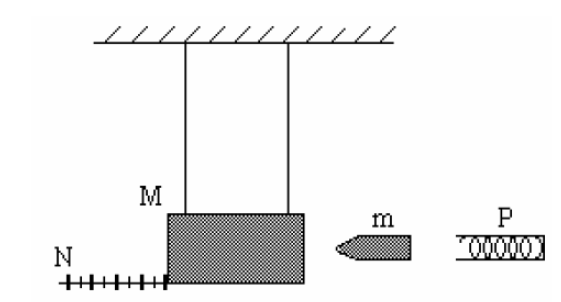
\includegraphics[scale=0.5]{схема}
 \end{figure}

\paragraph{Результаты прямых измерений и их обработки.}
\begin{itemize}
	\item Масса баллистического маятника: $ M=112\;\mbox{г} $ 
	\item Длина маятника: $ l=30\;\mbox{см}$
\end{itemize}
		
		\begin{table}[htb]
			\centering
		\caption{Измерения}
		\begin{tabular}{| c | c | c |}
			\hline
			№ & Масса пули $m_i$ (г) & Отклонение маятника $x_i$ (см) \\
			\hline
			1 & 11,53 & 9 \\
			\hline
			2 & 10,72 & 5 \\
			\hline
			3 & 3,74 & 2,5 \\
			\hline
		\end{tabular}
	\end{table}

\paragraph{Расчет результатов косвенных измерений.}
Пользуясь \hyperlink{formuls}{формулой (1)}, находим скорости пуль:
\begin{table}[!htb]
	\centering
	
	\begin{tabular}{|c|c|}
		\hline
		№ & Скорость пули $v_i$ ($\frac{\mbox{м}}{\mbox{с}}$) \\
		\hline
		1 &  5,51  \\
		\hline
		2 &  3,27  \\
		\hline
		3 & 4,42  \\
		\hline
	\end{tabular}
\end{table}

\paragraph{Расчет погрешностей измерений.}
$$ v=v(m,\;M,\;l,\;x)$$
$$ 
\Delta v=\sqrt{\left(\frac{\partial v}{\partial m}\Delta m\right)^2 + \left(\frac{\partial v}{\partial M}\Delta M\right)^2 + \left(\frac{\partial v}{\partial l}\Delta l\right)^2 + \left(\frac{\partial v}{\partial x}\Delta x\right)^2}
$$


	 $$\frac{\partial v}{\partial m}\Delta m =x\sqrt{\frac{g}{l}}\left(-\frac{M}{m^2}\right) \Delta m$$
	 $$ \frac{\partial v}{\partial M}\Delta M = \frac{x}{m}\sqrt{\frac{g}{l}}\cdot\Delta M$$
	 $$ \frac{\partial v}{\partial l}\Delta l = \frac{m+M}{m}\;x\sqrt{g}\left( -\frac{1}{2\sqrt{l^3}}\right) $$
	 $$ \frac{\partial v}{\partial x}\Delta x = \frac{m+M}{m}\sqrt{\frac{g}{l}}\cdot\Delta x$$

В итоге:

$$ \Delta v = \sqrt{\frac{x^2 g M^2}{l m^4}\Delta m^2 +  \frac{x^2 g}{m^2 l}\Delta M^2 + \frac{(m+M)^2 x^2 g}{4m^2 l^3}\Delta l^2 + \frac{(m+M)^2 g}{m^2 l}\Delta x^2}$$\\
$\Delta m = 0,01$ г\\
$ \Delta M = 0,1$ г\\
$ \Delta l =  5$ мм\\
$ \Delta x = 2 $ см
\begin{table}[htb]
	\centering
	\begin{tabular}{|c|c|}
		\hline
		№ & Погрешность скорости $\Delta v_i$ $\left( \frac{\mbox{м}}{\mbox{с}}\right) $\\
		\hline
		1 & 1,2 \\
		\hline
		2 & 1,3\\
		\hline
		3 &  3,5\\
		\hline
	\end{tabular}
\end{table}


\begin{table}[htb]
	\caption{\bf Окончательные результаты.}
	\centering
	\begin{tabular}{|c|c|}
		\hline
		№ & Скорость пули $v_i$ ($\frac{\mbox{м}}{\mbox{с}}$) \\
		\hline
		1 &  $\left( 5,5\pm1,2\right) $ \\
		\hline
		2 &  $\left( 3,3\pm1,3\right) $ \\
		\hline
		3 & $\left( 4,4\pm3,5\right) $ \\
		\hline
	\end{tabular}
\end{table}

\begin{figure}[!htb]
	\centering
	\caption{Зависимость скорости $v$ от $\sqrt{\frac{1}{m}}$}
\begin{tikzpicture}
	\begin{axis}[ minor tick num = 4, grid=major, xlabel = $\sqrt{\frac{1}{m}}$, ylabel = Скорость $v$ $\left( \frac{\mbox{м}}{\mbox{с}}\right) $]
		\addplot [ only marks, mark=*, error bars/.cd, y dir=both, y explicit]
		table [x=x, y=y, y error=y-err]{%
			x y y-err
			9.31 5.51 1.2 
			9.66 3.27 1.3
			16.35 4.42 3.5
			0 0 0
		};
	\end{axis}
\end{tikzpicture}
\end{figure}

\paragraph{Выводы и анализ результатов}
Мы 

\end{document}



